\chapter{TODO Results}
\label{ch:results}

In this chapter, we present the results of the decentralized ticketing system,
including interactions with smart contracts, the process of buying, gifting,
refunding, and validating tickets, and the associated blockchain transactions.

    [TODO mention sections]

As mentioned earlier, blockchain serves as a public ledger that records all
transactions. We deployed the smart contracts on a testnet to avoid the use of
real funds, allowing us to simulate mainnet operations without incurring risks
or costs. This was achieved using Foundry, and we developed scripts to populate
the system, which included deploying the smart contracts, adding an event
organizer, creating events, and adding ticket packages to each event.

Every network has an explorer that visualizes all transactions. Figure
\ref{fig:ticketchain_transactions} illustrates the transactions related to our
system.
\begin{figure}[H]
    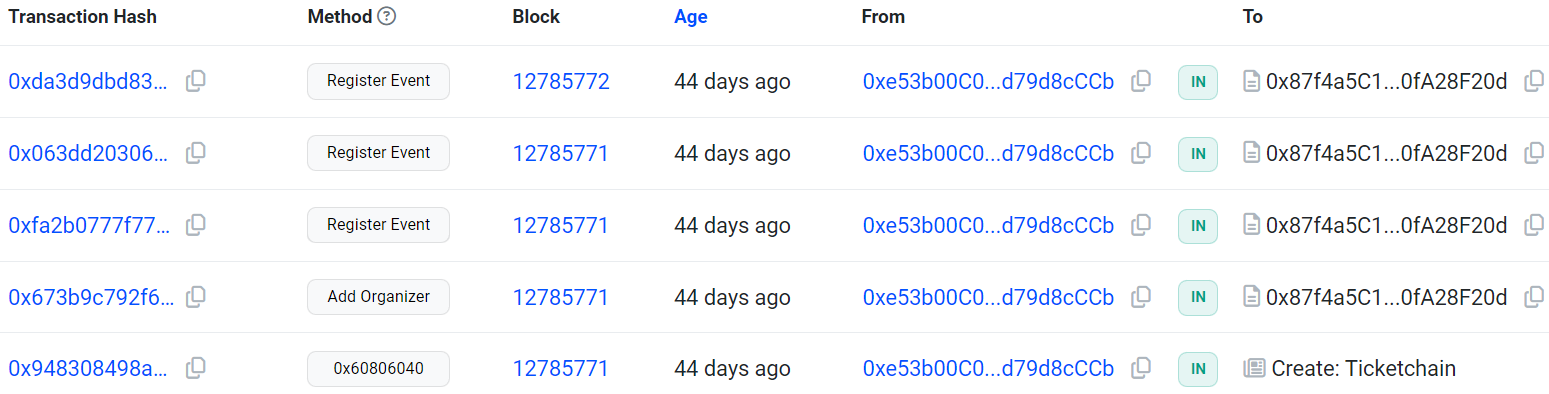
\includegraphics[width=\textwidth]{Ticketchain transactions.png}
    \centering
    \caption{Ticketchain transactions}
    \label{fig:ticketchain_transactions}
\end{figure}

This explorer allows us to track when the contract was deployed, the addition
of an organizer, and the creation of three events. This data is subsequently
loaded into the app, as shown earlier in Figure \ref{fig:home_page}.

\section{Buying Tickets}
\label{sec:buy_tickets}

To purchase tickets, users follow the procedure outlined in Section
\ref{subsec:events}. Figures \ref{fig:home_page} and \ref{fig:tickets_page}
show two available events, although there are three in total. We will now
demonstrate the process of buying tickets for the third event, which has one
available package containing 100 tickets, as seen in Figure
\ref{fig:buy_tickets_event}.

\begin{figure}[H]
    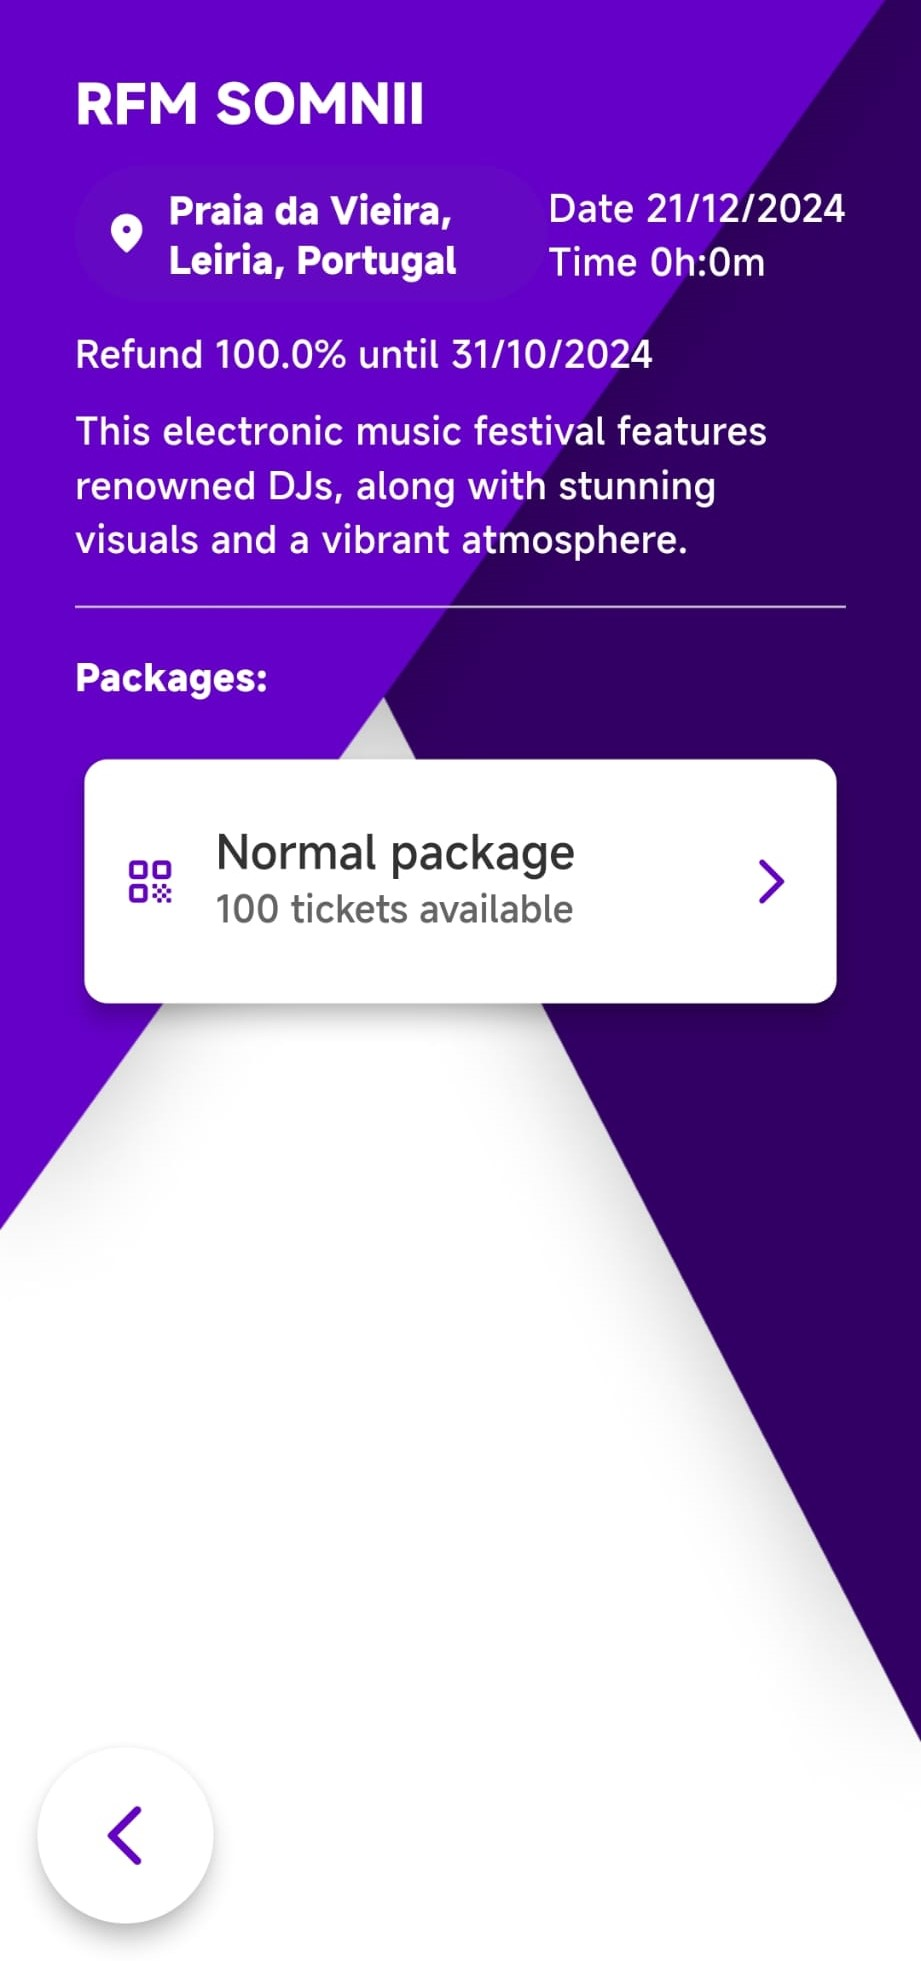
\includegraphics[width=\textwidth/3,frame]{Event page 2.jpg}
    \centering
    \caption{Third event page}
    \label{fig:buy_tickets_event}
\end{figure}

After selecting the package, the user is prompted to choose the number of
tickets to purchase. In this case, we will buy 3 tickets, as illustrated in
Figure \ref{fig:buy_tickets_prompt_2}.

\begin{figure}[H]
    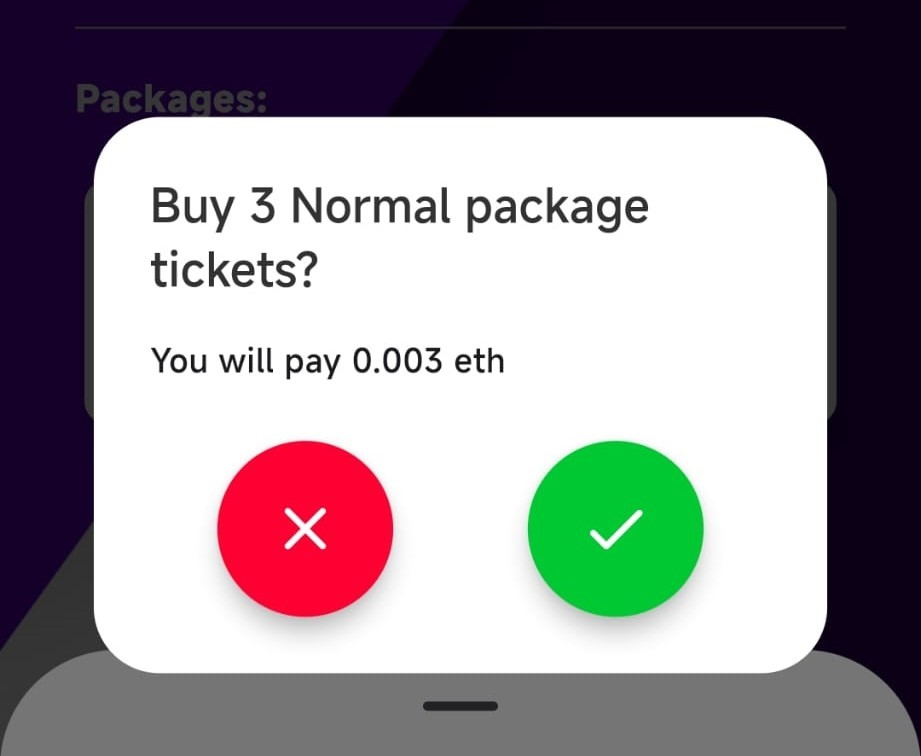
\includegraphics[width=\textwidth/3,frame]{Buy tickets prompt 2.jpg}
    \centering
    \caption{Prompt to buy 3 tickets}
    \label{fig:buy_tickets_prompt_2}
\end{figure}

Upon confirmation, the user's wallet opens, and the transaction is displayed
for approval (Figure \ref{fig:buy_tickets_transaction}).

\begin{figure}[H]
    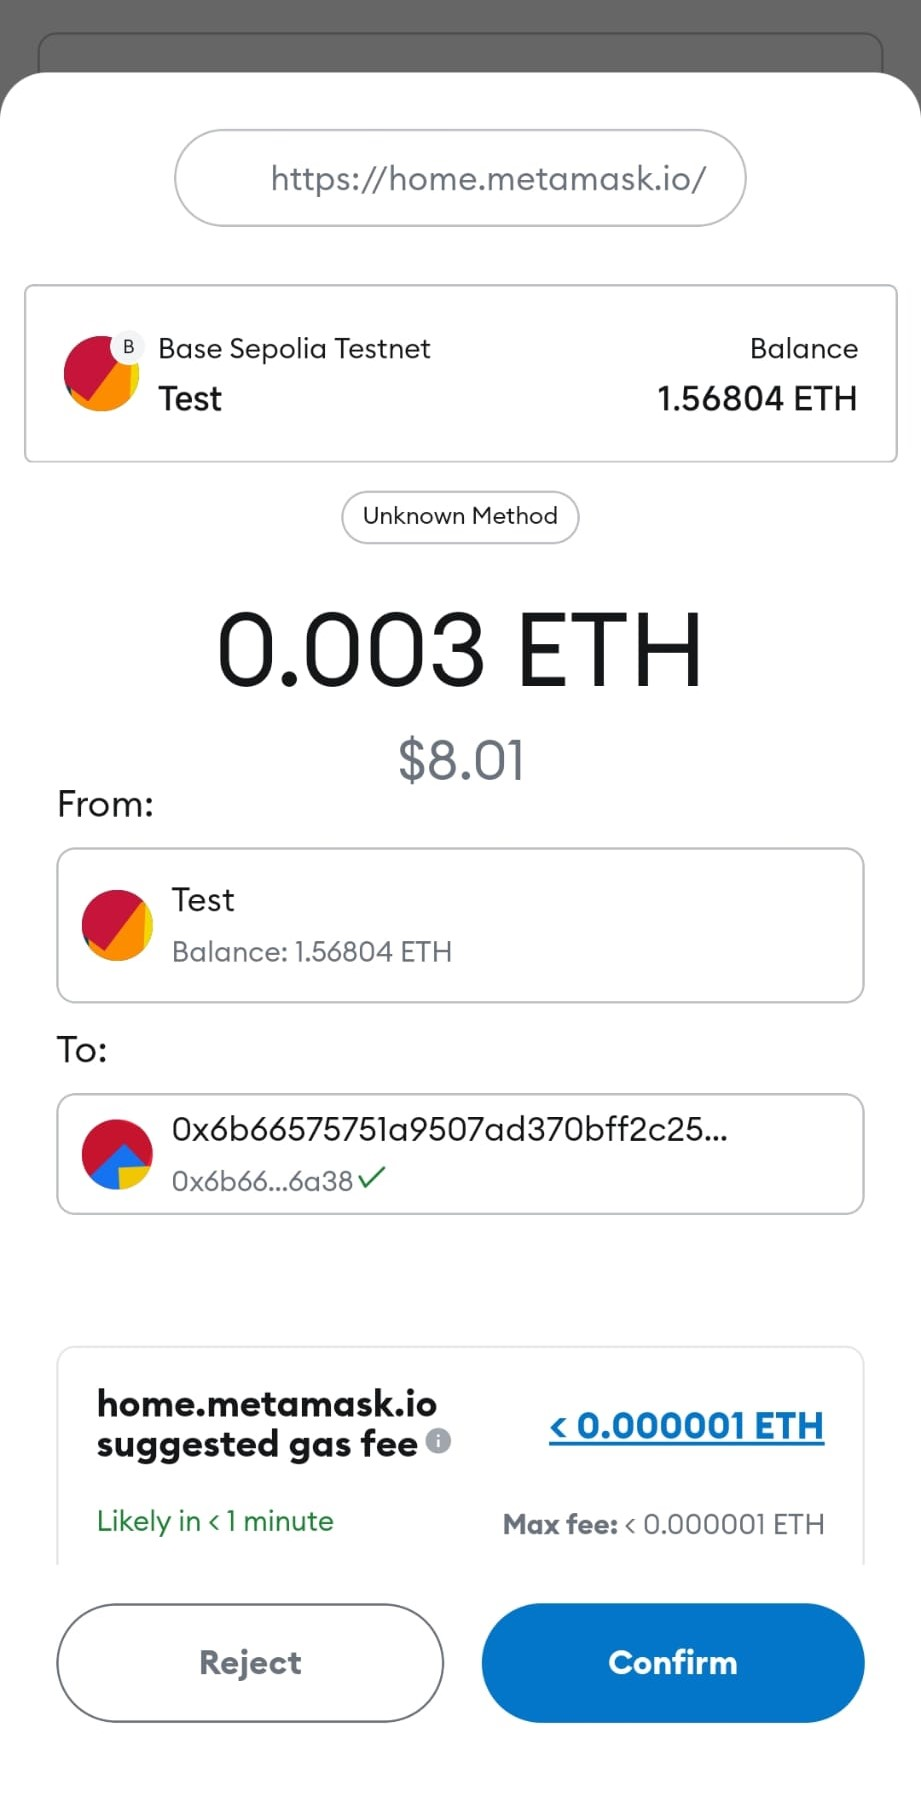
\includegraphics[width=\textwidth/3,frame]{MetaMask transaction prompt 2.jpg}
    \centering
    \caption{Buy 3 tickets transaction prompt}
    \label{fig:buy_tickets_transaction}
\end{figure}

The user sends 0.003 ETH to complete the purchase. After successful payment,
the profile page updates to reflect the addition of the third event and 3
purchased tickets (Figure \ref{fig:profile_page_2}).

\begin{figure}[H]
    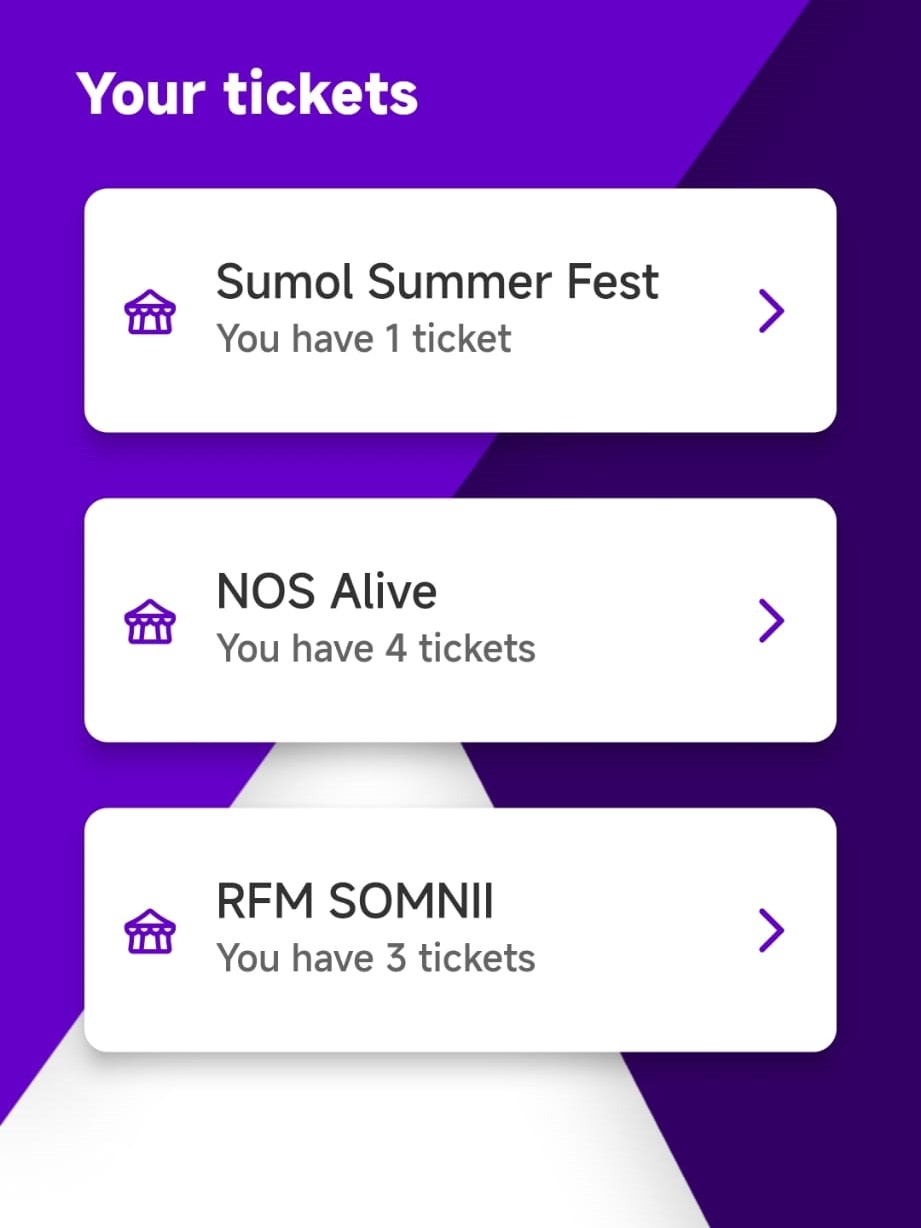
\includegraphics[width=\textwidth/3,frame]{Profile page 2.jpg}
    \centering
    \caption{Profile page showing tickets for the third event}
    \label{fig:profile_page_2}
\end{figure}

Returning to the event page, we see that the number of available tickets has
decreased to 97, as shown in Figure \ref{fig:buy_tickets_event_2}.

\begin{figure}[H]
    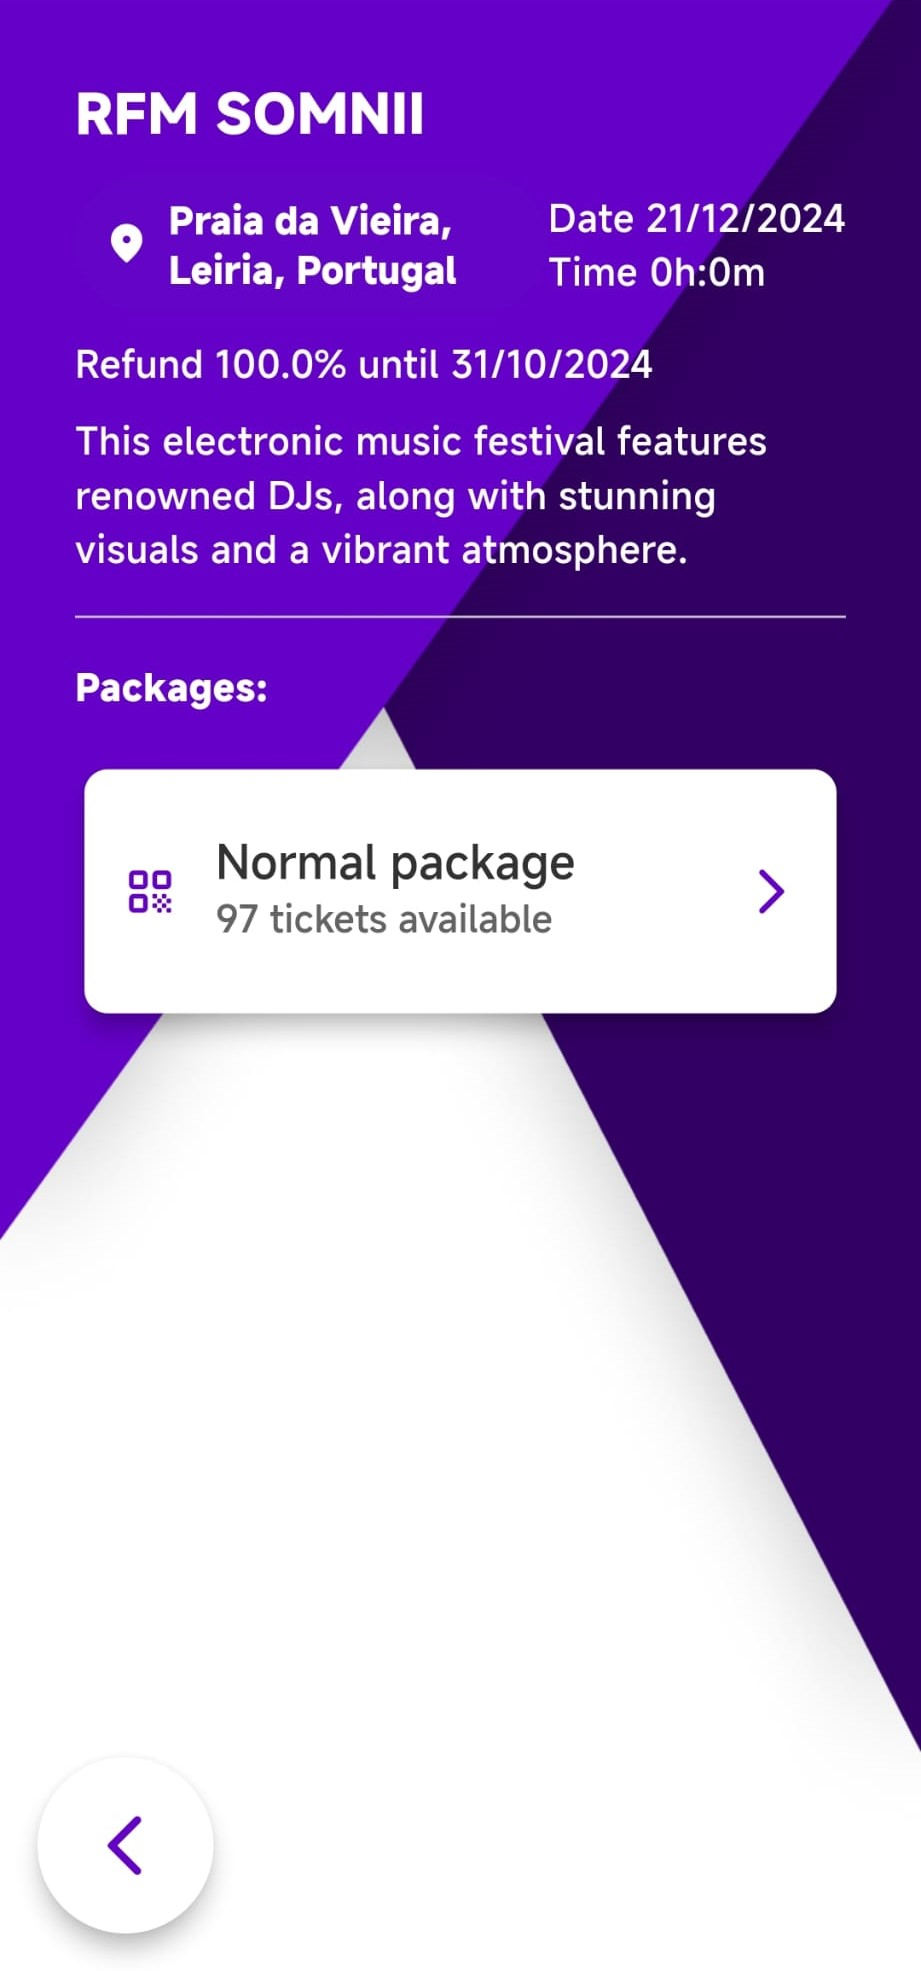
\includegraphics[width=\textwidth/3,frame]{Event page 3.jpg}
    \centering
    \caption{Third event page with 97 tickets remaining}
    \label{fig:buy_tickets_event_2}
\end{figure}

The blockchain explorer shows the associated transaction, as displayed in
Figure \ref{fig:user_transactions}.

\begin{figure}[H]
    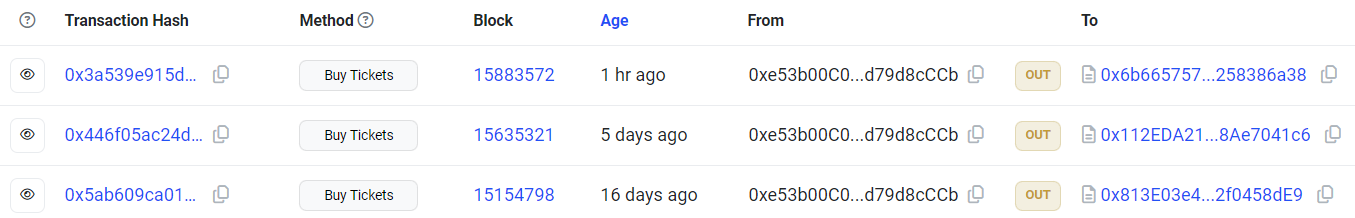
\includegraphics[width=\textwidth]{User transactions.png}
    \centering
    \caption{User's transaction history}
    \label{fig:user_transactions}
\end{figure}

By selecting the transaction hash, we can view the transaction details (Figure
\ref{fig:buy_tickets_transaction_details}).

\begin{figure}[H]
    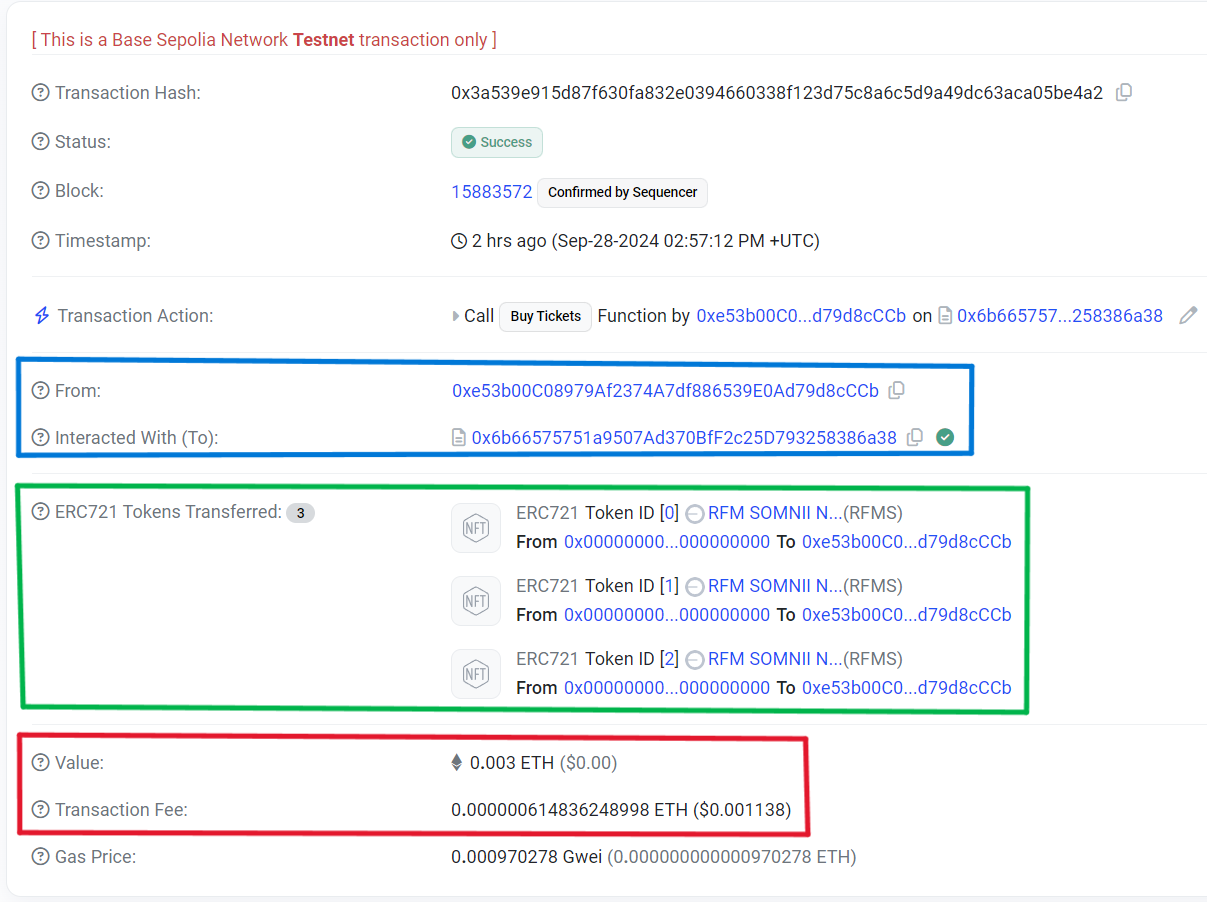
\includegraphics[width=\textwidth]{Buy tickets transaction details.png}
    \centering
    \caption{Details of the buy tickets transaction}
    \label{fig:buy_tickets_transaction_details}
\end{figure}

The key information includes the following:
\paragraph{Blue box:} The addresses involved in the transaction, where the \textit{From} field shows
the user's address and the \textit{To} field shows the event contract address.
\paragraph{Green box:} The NFTs (tickets) transferred, showing that IDs 0, 1, and 2 were minted and
assigned to the user.
\paragraph{Red box:} The amount of ETH sent (0.003 ETH) and the network fee paid for the
transaction.

\section{Gifting Tickets}
\label{sec:gift_tickets}

To gift tickets, the user selects the tickets to transfer, as shown in Figure
\ref{fig:gift_tickets_prompt}.

\begin{figure}[H]
    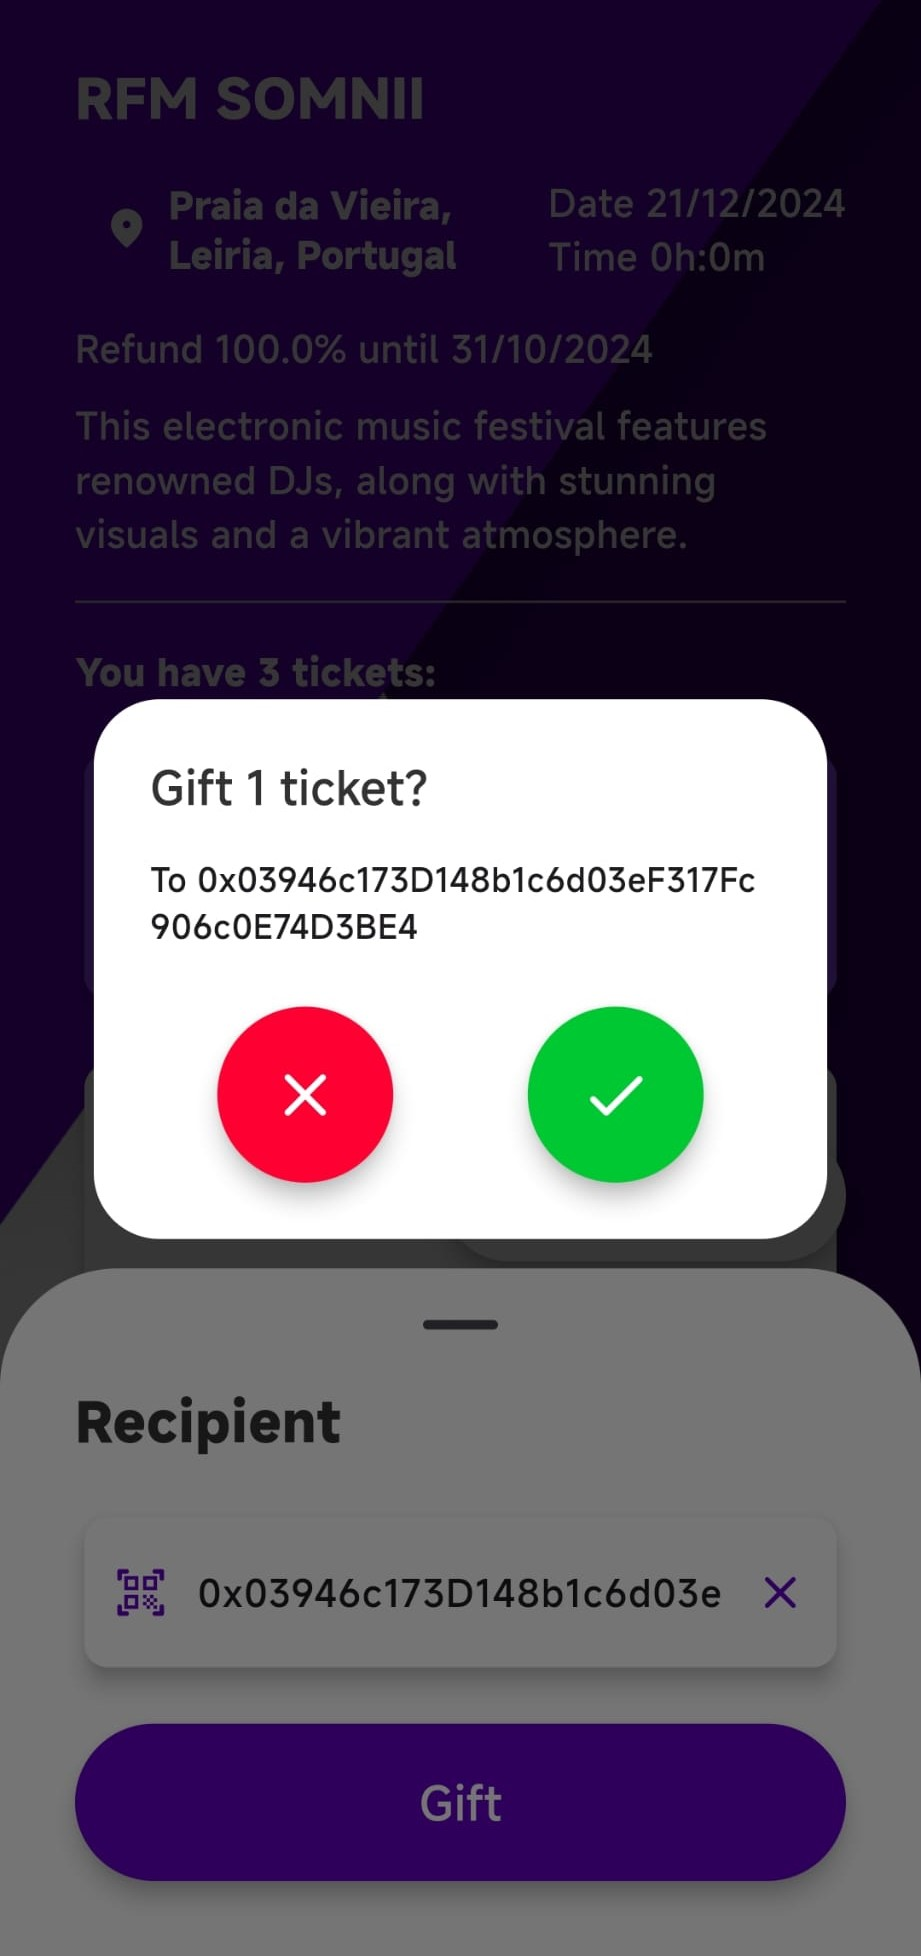
\includegraphics[width=\textwidth/3,frame]{Gift tickets prompt.jpg}
    \centering
    \caption{Prompt to gift tickets}
    \label{fig:gift_tickets_prompt}
\end{figure}

After the transaction is executed, we log out and authenticate with the
recipient's wallet to confirm the successful transfer (Figure
\ref{fig:profile_page_3}).

\begin{figure}[H]
    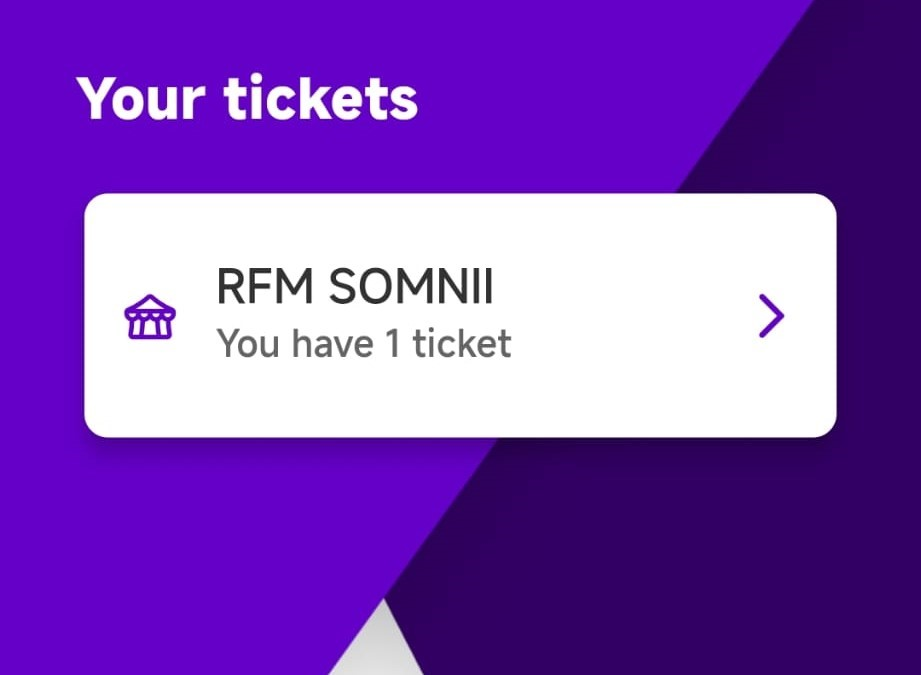
\includegraphics[width=\textwidth/3,frame]{Profile page 3.jpg}
    \centering
    \caption{Profile page showing gifted tickets}
    \label{fig:profile_page_3}
\end{figure}

The blockchain explorer records the gifting transaction details, as shown in
Figure \ref{fig:gift_tickets_transaction_details}.

\begin{figure}[H]
    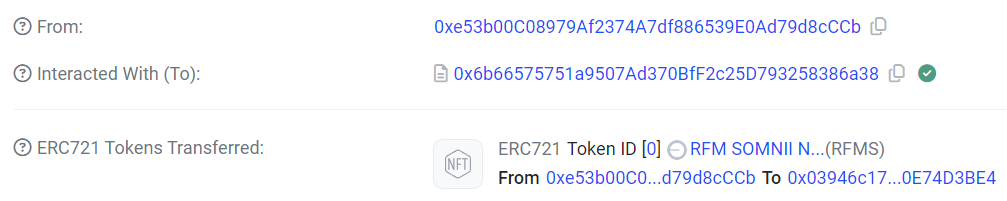
\includegraphics[width=\textwidth]{Gift tickets transaction details.png}
    \centering
    \caption{Details of the gift tickets transaction}
    \label{fig:gift_tickets_transaction_details}
\end{figure}

The transaction shows that the NFT with ID 0 was transferred from the original
user's address to the recipient's address.

\section{Refunding Tickets}
\label{sec:refund_tickets}

The refund process mirrors the gifting process, except that the tickets are
burned in exchange for a refund. Figure \ref{fig:refund_tickets_prompt} shows
the prompt, indicating the refund amount, which in this case is 100\%.

\begin{figure}[H]
    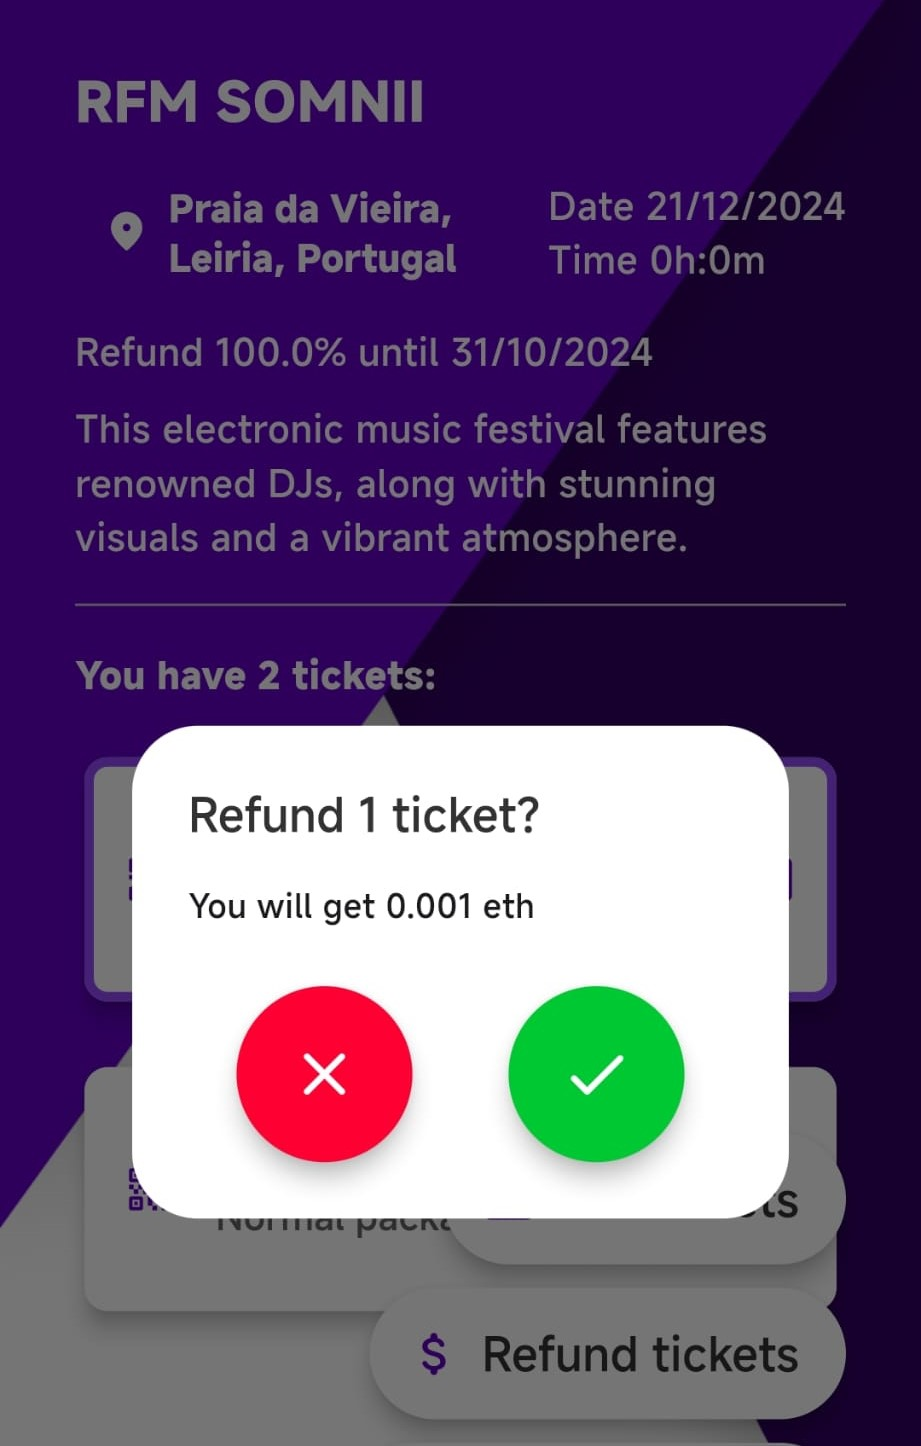
\includegraphics[width=\textwidth/3,frame]{Refund tickets prompt.jpg}
    \centering
    \caption{Refund tickets prompt}
    \label{fig:refund_tickets_prompt}
\end{figure}

Once the transaction is executed, the blockchain records the details, as seen
in Figure \ref{fig:refund_tickets_transaction_details}.

\begin{figure}[H]
    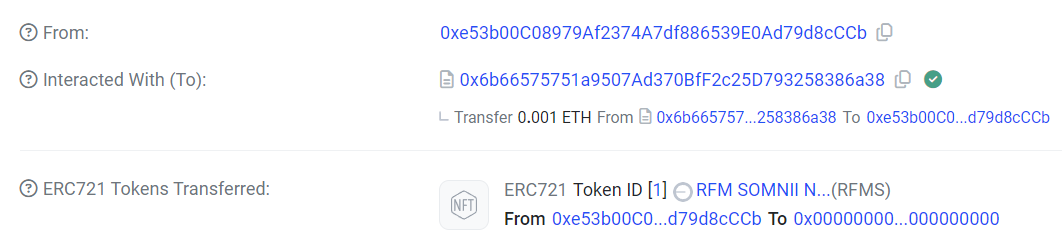
\includegraphics[width=\textwidth]{Refund tickets transaction details.png}
    \centering
    \caption{Details of the refund tickets transaction}
    \label{fig:refund_tickets_transaction_details}
\end{figure}

The NFT with ID 1 is sent to the null address (0x00\dots00), indicating it has
been burned. Simultaneously, the user receives a refund of 0.001 ETH, and the
event page reflects an increase in available tickets from 97 to 98 (Figure
\ref{fig:refund_tickets_event}).

\begin{figure}[H]
    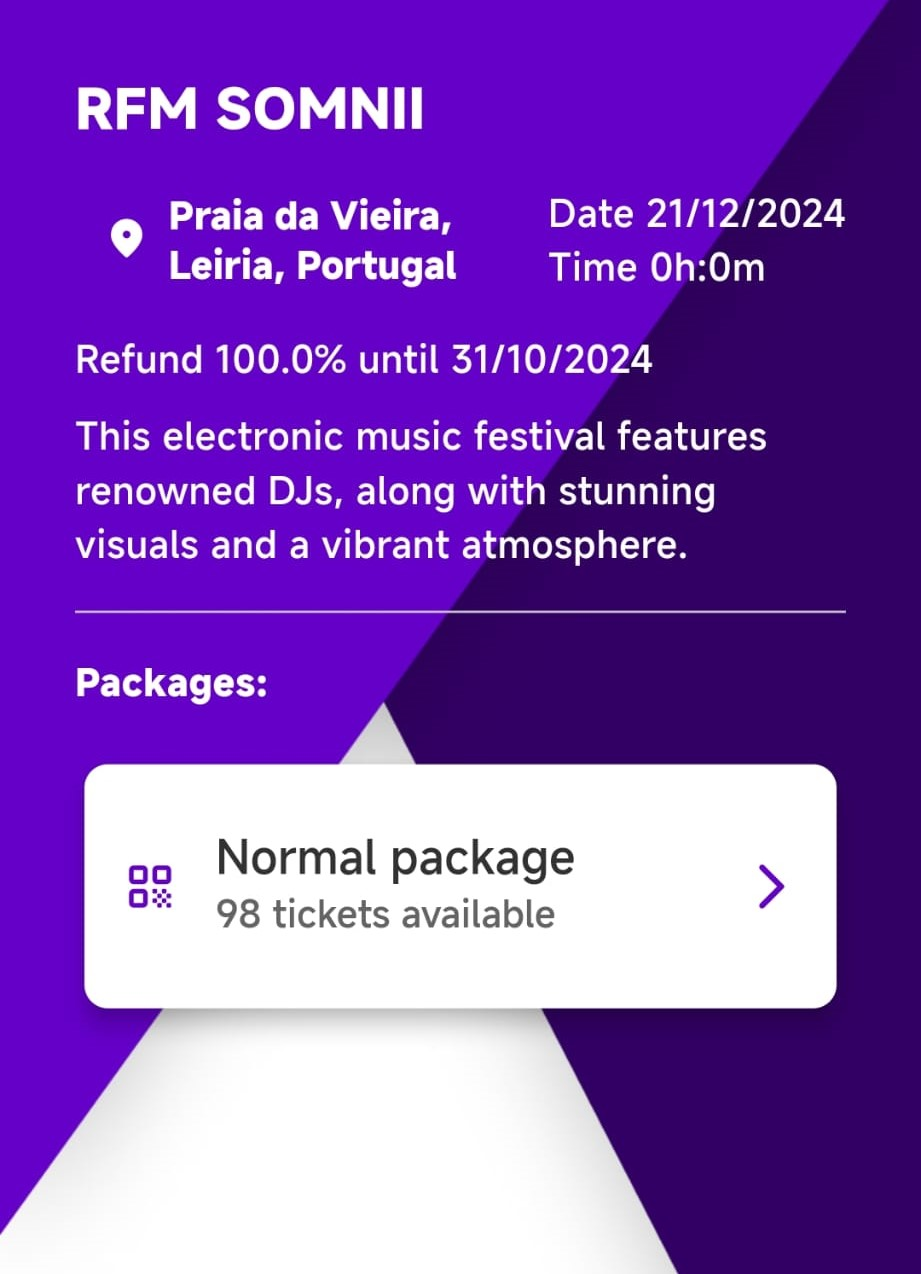
\includegraphics[width=\textwidth/3,frame]{Event page 4.jpg}
    \centering
    \caption{Third event page with 98 tickets available}
    \label{fig:refund_tickets_event}
\end{figure}

\section{Validating Tickets}
\label{sec:validate_tickets}

As shown in the Section \ref{sec:ticket_validation}, the ticket validation
process happens between the user and the validator. When the user selects the
tickets he wants to validate, he'll be prompted to scan the QR code generated
by the validator. The Figure \ref{fig:validate_tickets_qr_validator} shows the
QR code generated by the validator.

\begin{figure}[H]
    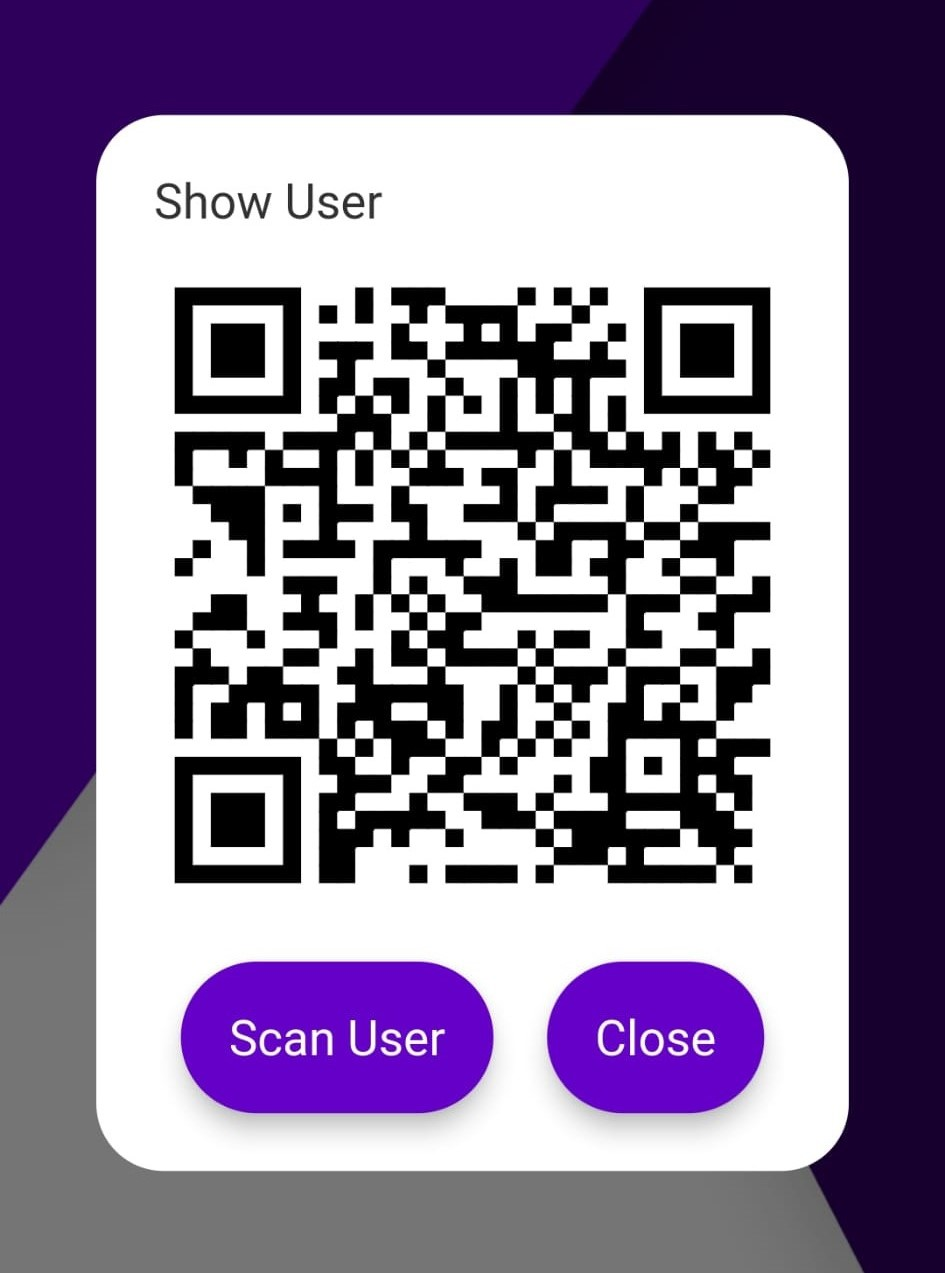
\includegraphics[width=\textwidth/3,frame]{Validate tickets qr validator.jpg}
    \centering
    \caption{QR code generated by the validator}
    \label{fig:validate_tickets_qr_validator}
\end{figure}

Once the QR code is read, the user's wallet will open, and will ask the user to
sign the message. The Figure \ref{fig:validate_tickets_sign_message} shows the
message that the user will sign.

\begin{figure}[H]
    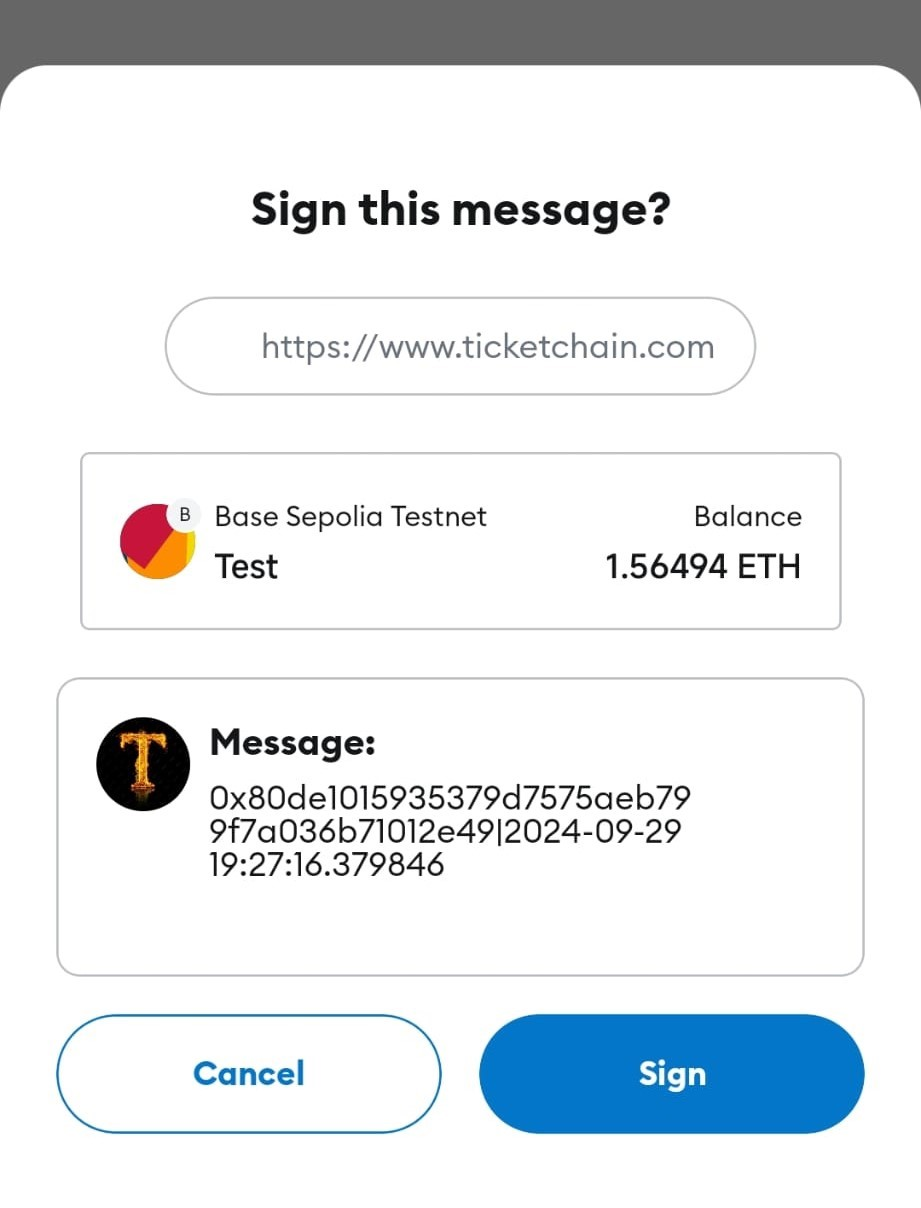
\includegraphics[width=\textwidth/3,frame]{Validate tickets sign message.jpg}
    \centering
    \caption{Message that the user will sign}
    \label{fig:validate_tickets_sign_message}
\end{figure}

We see that the message has the validator's address with the date. After the
users signs it, the user will display a QR code with the necessary information
for the validator, as shown in the Figure \ref{fig:validate_tickets_qr_user}.

\begin{figure}[H]
    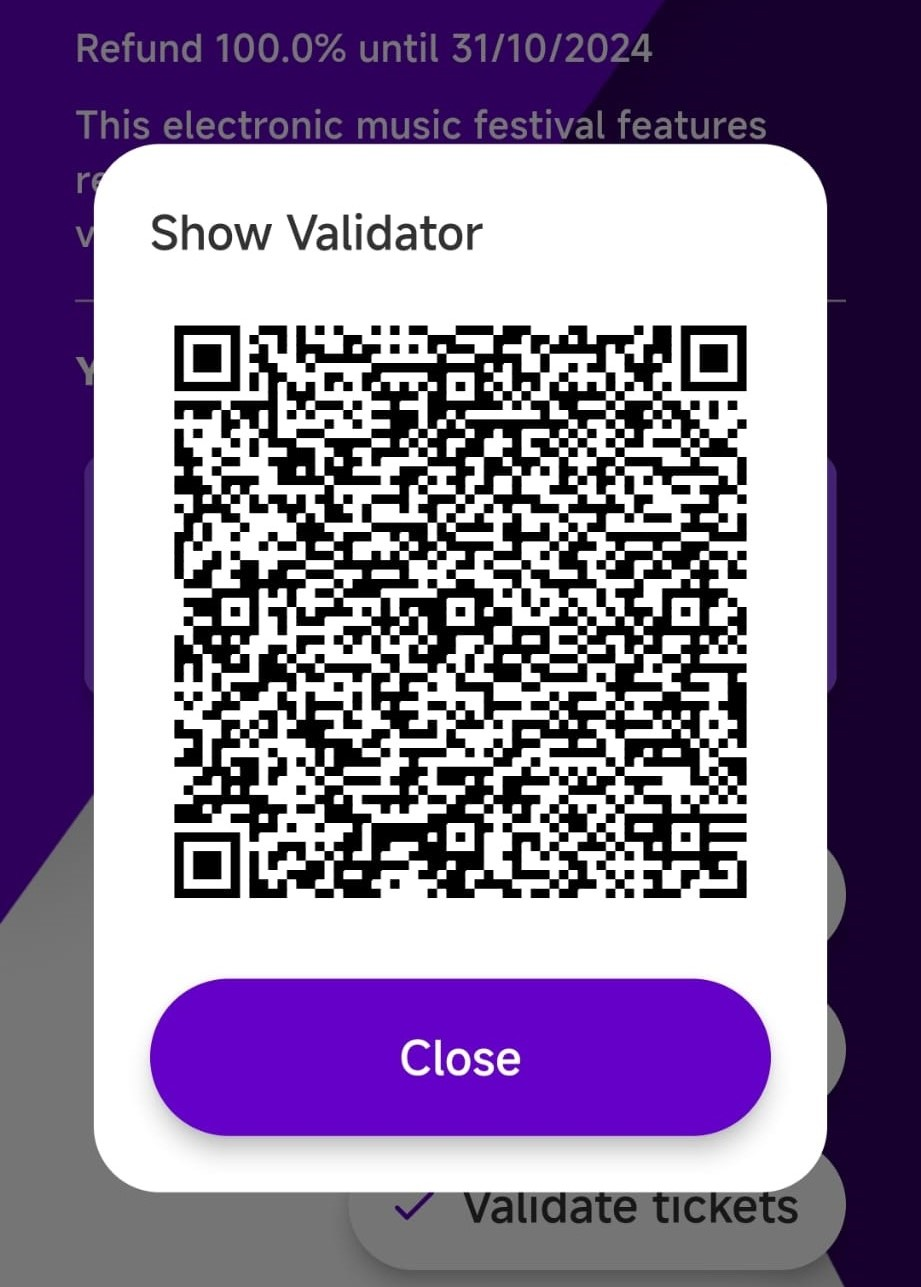
\includegraphics[width=\textwidth/3,frame]{Validate tickets qr user.jpg}
    \centering
    \caption{QR code generated by the user}
    \label{fig:validate_tickets_qr_user}
\end{figure}

After the validator reads the QR code, he'll check if everything is correct and
finishes the validation process, which then shows the prompt in the Figure
\ref{fig:validate_tickets_success}.

\begin{figure}[H]
    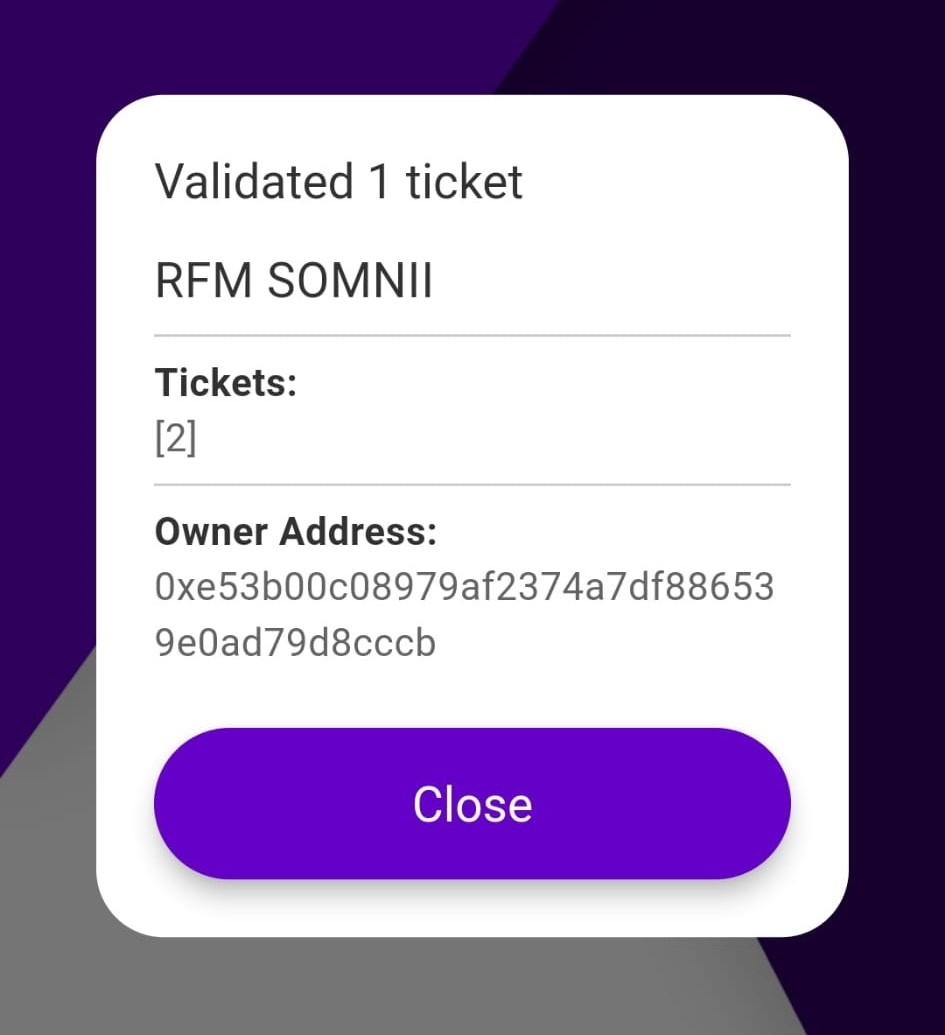
\includegraphics[width=\textwidth/3,frame]{Validate tickets success.jpg}
    \centering
    \caption{Validation success prompt}
    \label{fig:validate_tickets_success}
\end{figure}

We can verify the ticket is validated since now the user sees its ticket with a
checkmark, as the Figure \ref{fig:validate_tickets_validated} shows.

\begin{figure}[H]
    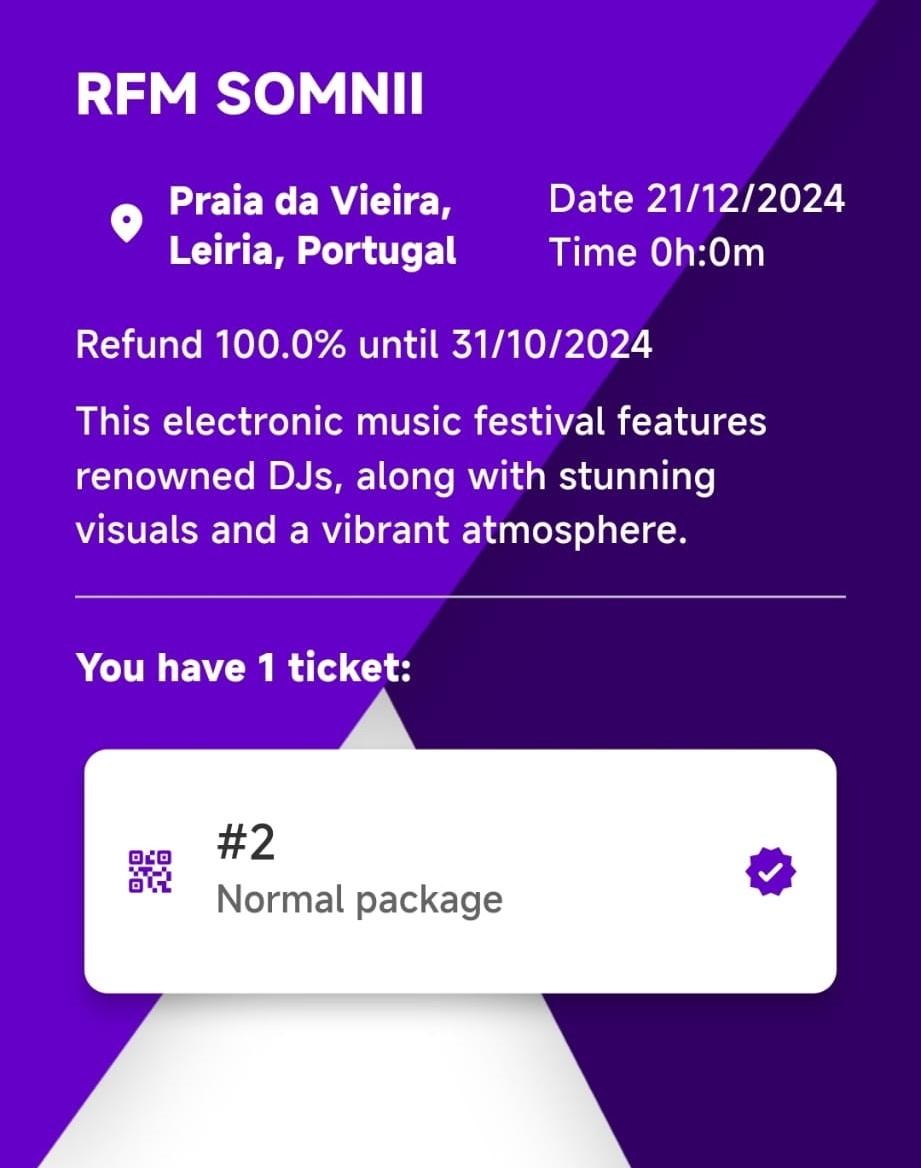
\includegraphics[width=\textwidth/3,frame]{Validate tickets validated.jpg}
    \centering
    \caption{Validated ticket}
    \label{fig:validate_tickets_validated}
\end{figure}